\documentclass[11pt]{article}
% =========================================================================
% SHARED STYLE FILE for 11_Master_Projects reports
% Visual style follows 0_Thesis_Submission/24m0553_AK_Gaurav_Mtech_Report.pdf:
% serif body font, blue hyperlinked TOC/links, ruled section headings,
% IITB-style title page, formal academic report structure.
% =========================================================================

\usepackage[a4paper,margin=1in]{geometry}
\usepackage{xcolor}
\usepackage{graphicx}
\graphicspath{{../images/}}
\usepackage{amsmath,amssymb}
\usepackage{booktabs}
\usepackage{caption}
\usepackage{float}
\usepackage[hidelinks]{hyperref}
\usepackage{titlesec}
\usepackage{enumitem}
\usepackage{setspace}
\usepackage[T1]{fontenc}
\usepackage{lmodern}
\usepackage{microtype}

% Every \includegraphics call is automatically framed with a thin black
% border (matches the printed look of figures/photos/charts in the source
% reports). \oldincludegraphics is kept available for institutional
% logos/seals on title pages, which should remain unframed.
\let\oldincludegraphics\includegraphics
\setlength{\fboxsep}{1pt}
\setlength{\fboxrule}{0.6pt}
\renewcommand{\includegraphics}[2][]{\fbox{\oldincludegraphics[#1]{#2}}}

\definecolor{thesisblue}{RGB}{0,0,205}
\hypersetup{
  colorlinks=true,
  linkcolor=thesisblue,
  urlcolor=thesisblue,
  citecolor=thesisblue,
  filecolor=thesisblue
}

\onehalfspacing
\setlength{\parskip}{6pt}
\setlength{\parindent}{0pt}

\titleformat{\section}
  {\normalfont\Large\bfseries}{\thesection}{1em}{}
\titleformat{\subsection}
  {\normalfont\large\bfseries}{\thesubsection}{1em}{}
\titleformat{\subsubsection}
  {\normalfont\normalsize\bfseries}{\thesubsubsection}{1em}{}

\newcommand{\reportTitlePage}[7]{%
  % #1 = Report title
  % #2 = Course code & name (e.g. "CE 605: Applied Statistics")
  % #3 = Subtitle/topic line (e.g. "Project Report 2: Network Analysis")
  % #4 = Author block (can be multi-line with \\ for group projects)
  % #5 = Supervisor name(s)
  % #6 = Programme line (e.g. "M.Tech in Transportation Systems Engineering")
  % #7 = Month/Year
  \begin{titlepage}
    \centering
    \vspace*{0.5cm}
    {\large\bfseries #2}\par
    \vspace{0.3cm}
    {\Large\bfseries #3}\par
    \vspace{1.2cm}
    {\Huge\bfseries #1}\par
    \vspace{1.5cm}
    \oldincludegraphics[width=3.2cm]{../../assets/iitb_logo.png}\par
    \vspace{1.2cm}
    Submitted by:\par
    \vspace{0.2cm}
    {\bfseries #4}\par
    \vspace{0.8cm}
    Under the Supervision of\par
    \vspace{0.2cm}
    {\bfseries #5}\par
    \vspace{1.2cm}
    #6\par
    Department of Civil Engineering\par
    \textbf{Indian Institute of Technology Bombay}\par
    Mumbai -- 400076, India\par
    \vspace{0.3cm}
    #7\par
  \end{titlepage}
}

\newcommand{\reportAbstract}[1]{%
  \section*{Abstract}
  #1
  \vspace{0.5cm}
}

\usepackage{longtable}

\title{Geometric Design and Analysis of the Simaria--Matihani Greenfield Bypass Road, Begusarai District, Bihar}
\author{Abhijeet Kumar Gaurav}
\date{}

\begin{document}

\reportTitlePage
  {Geometric Design and Analysis of the Simaria--Matihani Greenfield Bypass Road, Begusarai District, Bihar}
  {CE 773: Geometric Design and Analysis of High-Speed Roadways}
  {Course Project}
  {Abhijeet Kumar Gaurav \\ Roll No.: 24M0553}
  {Prof. Avijit Maji}
  {M.Tech in Transportation Systems Engineering}
  {Spring 2025}

\pagenumbering{roman}

\reportAbstract{
Begusarai district in Bihar hosts three major industrial assets, namely the IOCL Barauni Refinery, the
NTPC Barauni Thermal Power Station, and the HURL Barauni Fertilizer Plant, yet its only regional
arterial, NH-31, suffers chronic congestion, a low average speed of 18~km/h against an 80~km/h design
speed, and 142 recorded fatal accidents in 2024. This report presents the geometric design of a
proposed greenfield bypass connecting Simaria, Shihma village, and Matihani, intended to divert
industrial and through traffic away from the congested urban core of Begusarai. The original scope of
the project called for three candidate alignments, but owing to the time available for this coursework
exercise, full geometric design was carried through to completion for two of them: a 4-lane, 100~km/h
alignment (Alignment 1) and a 2-lane, 80~km/h alignment (Alignment 3) routed to minimise land
acquisition through the Makor habitation area. A third, 4-lane, 80~km/h option (Alignment 2) was
explored at the routing and superelevation stage in AutoCAD Civil 3D using a Digital Elevation Model
(DEM) of the corridor, but was not carried through to full corridor modelling and earthwork
quantification. For the two completed alignments, horizontal alignments, spiral transitions,
superelevation, vertical profiles, and corridor cross-sections were generated in accordance with
IRC:73-1980 and IRC:SP:84 guidelines, and cut-fill earthwork volumes were quantified along each
alignment. The resulting designs demonstrate a terrain-responsive, standards-compliant
bypass geometry that supports the stated policy objective of reducing NH-31 traffic volume by
38--42\% while improving industrial and agricultural connectivity in the region.

\vspace{0.3cm}
\noindent\textbf{Keywords:} Highway Geometric Design; Greenfield Bypass; AutoCAD Civil 3D; Horizontal
and Vertical Alignment; Superelevation; IRC:73-1980; Earthwork Analysis
}

\newpage
\tableofcontents
\newpage
\pagenumbering{arabic}

\section{Introduction and Study Area}

\subsection{Project Background}
The Simaria to Lakhminia bypass is part of the Government of Bihar's greenfield initiative to reduce
traffic congestion and improve regional connectivity around Begusarai. The proposed alignment begins
at Simaria, passes through Bind Toli, Shihma, and Matihani, and terminates at Lakhminia. As a
greenfield project, the bypass is to be constructed on new land to accommodate rising traffic demand
rather than widening the existing corridor.

\textbf{Alignment definition:}
\begin{itemize}
  \item \textbf{Start point:} Simaria ($25.44816^\circ$N, $85.92636^\circ$E)
  \item \textbf{End point:} Matihani ($25.421^\circ$N, $86.075^\circ$E)
  \item \textbf{Intermediate node:} Shihma village ($25.433^\circ$N, $86.012^\circ$E)
  \item \textbf{Total length:} Between 10--20~km (Phase~I: Simaria--Shihma--Matihani)
  \item \textbf{Future expansion:} A Phase~II extension to Ballia ($25.387^\circ$N, $86.131^\circ$E)
  has also been proposed.
\end{itemize}

\begin{figure}[H]
  \centering
  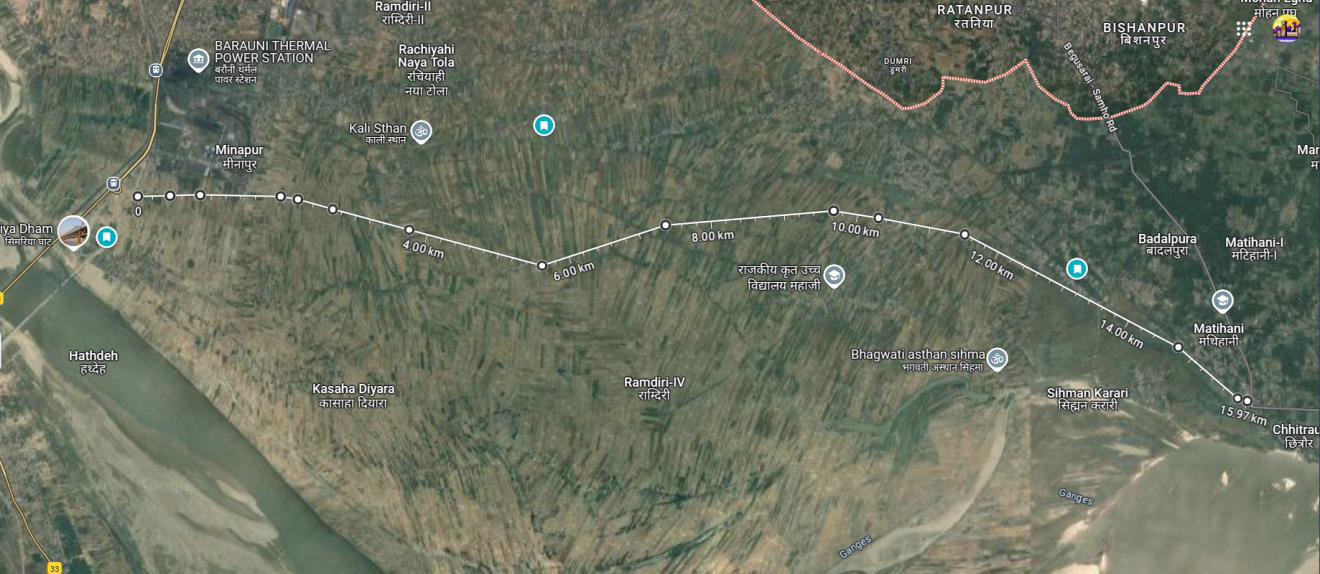
\includegraphics[width=0.85\textwidth]{fig_route_overview.png}
  \caption{Satellite overview of the Simaria--Shihma--Matihani bypass corridor.}
\end{figure}

According to the preliminary project brief, the bypass is expected to decongest NH-31 by diverting
40\% of commercial traffic away from Begusarai's urban core while connecting critical industrial and
agricultural zones. For the purposes of this coursework exercise, the actual Bihar government proposal
(the Simaria--Ballia Bypass Road) has been broken into two design phases, of which this report covers
Phase~I.

\subsection{Begusarai: An Emerging Urban-Industrial Hub}
Begusarai district, sometimes described as the ``Industrial Capital of Bihar,'' hosts three pillars of
the regional economy:

\begin{enumerate}
  \item \textbf{Indian Oil Corporation Limited (IOCL) Barauni Refinery}, with a capacity of 6 million
  metric tonnes/year, generating 35\% of Bihar's petroleum products.
  \item \textbf{Barauni Thermal Power Station (NTPC)}, with an installed capacity of 720~MW, supplying
  power to 12 districts.
  \item \textbf{Barauni Fertilizer Plant (HURL)}, with an annual production of 3.85 lakh metric tonnes
  of urea.
\end{enumerate}

The district's population is estimated at 1.9 million (2025), growing at a CAGR of 2.8\% (2011--2025)
against Bihar's state-wide average of 2.3\%. Simaria itself sits within the Barauni Industrial Complex,
on predominantly flat terrain well suited to alignment design, but the area is prone to seasonal
flooding owing to its proximity to the Ganga river.

\subsection{Existing Transportation Network and Challenges}
Table~\ref{tab:routes} summarises the key routes currently serving the study area.

\begin{table}[H]
  \centering
  \caption{Key existing routes in the Begusarai study area (2025 condition).}
  \label{tab:routes}
  \begin{tabular}{@{}llll@{}}
    \toprule
    \textbf{Route} & \textbf{Type} & \textbf{Condition} & \textbf{Peak-hour traffic (PCU/hr)} \\
    \midrule
    NH-31 (Urban) & 4-lane & Poor (PCI: 2.1/5) & 4,200 \\
    SH-78 & 2-lane & Fair (PCI: 3.4/5) & 1,850 \\
    Barauni--Begusarai Road & 2-lane & Critical & 3,100 \\
    \bottomrule
  \end{tabular}
\end{table}

\textbf{Identified problems:}
\begin{itemize}
  \item \textbf{Chronic congestion:} Daily traffic jams at Kapasia Chowk (NH-31/SH-78 junction); average
  vehicle speed of 18~km/h against a design speed of 80~km/h.
  \item \textbf{Safety issues:} 142 fatal accidents recorded in 2024 on the NH-31 Begusarai stretch,
  with black spots at Khatopur Chowk (23 accidents) and IOCL Gate No.~2 (17 accidents).
  \item \textbf{Connectivity gaps:} No direct link between the industrial zone (Simaria) and
  agricultural markets (Matihani).
\end{itemize}

Two interventions are already under way, namely the 4.3~km Begusarai Elevated Road (Kapasia Chowk to
Jail Chowk, completion expected December 2025) and a proposed Patna--Purnia Expressway link to the
Bakhri Industrial Park, but neither addresses regional connectivity in the Simaria area, and unmet
needs remain for last-mile connectivity to Shihma's agro-processing units and emergency access for
NTPC's coal transportation.

\subsection{Project Objectives and Expected Outcomes}
\textbf{Primary objectives:}
\begin{enumerate}
  \item Reduce NH-31 traffic volume by 38--42\% through diversion.
  \item Cut travel time on the Simaria--Ballia corridor from 82 minutes to 32 minutes.
  \item Enable 24/7 movement of oversized cargo for IOCL/NTPC.
  \item Connect currently unserved villages to the district headquarters.
\end{enumerate}

\textbf{Anticipated benefits} (per the proposed project brief and supporting articles):
\begin{itemize}
  \item \emph{Economic:} an estimated Rs.~2,300~crore/year in logistics-cost savings (FICCI
  2025 estimate), and a 15\% increase in fertilizer-plant output through more reliable coal supply.
  \item \emph{Social:} a projected 45\% reduction in road fatalities, and 22 new schools brought within
  a 30-minute access radius.
  \item \emph{Environmental:} an estimated 18,000 tonnes CO\textsubscript{2}/year reduction via shorter
  routes, and 32~ha of green belt along the bypass.
\end{itemize}

\subsection{Villages Along the Route}
The Simaria--Shihma bypass alignment passes through several key settlements, including Shihma (pincode
851129, Matihani block) and Malhipur (pincode 851118, under the Barauni Panchayat Samiti). These
villages stand to benefit directly from improved market access, reduced travel times, and easier
transportation of both agricultural produce and industrial goods.

\begin{figure}[H]
  \centering
  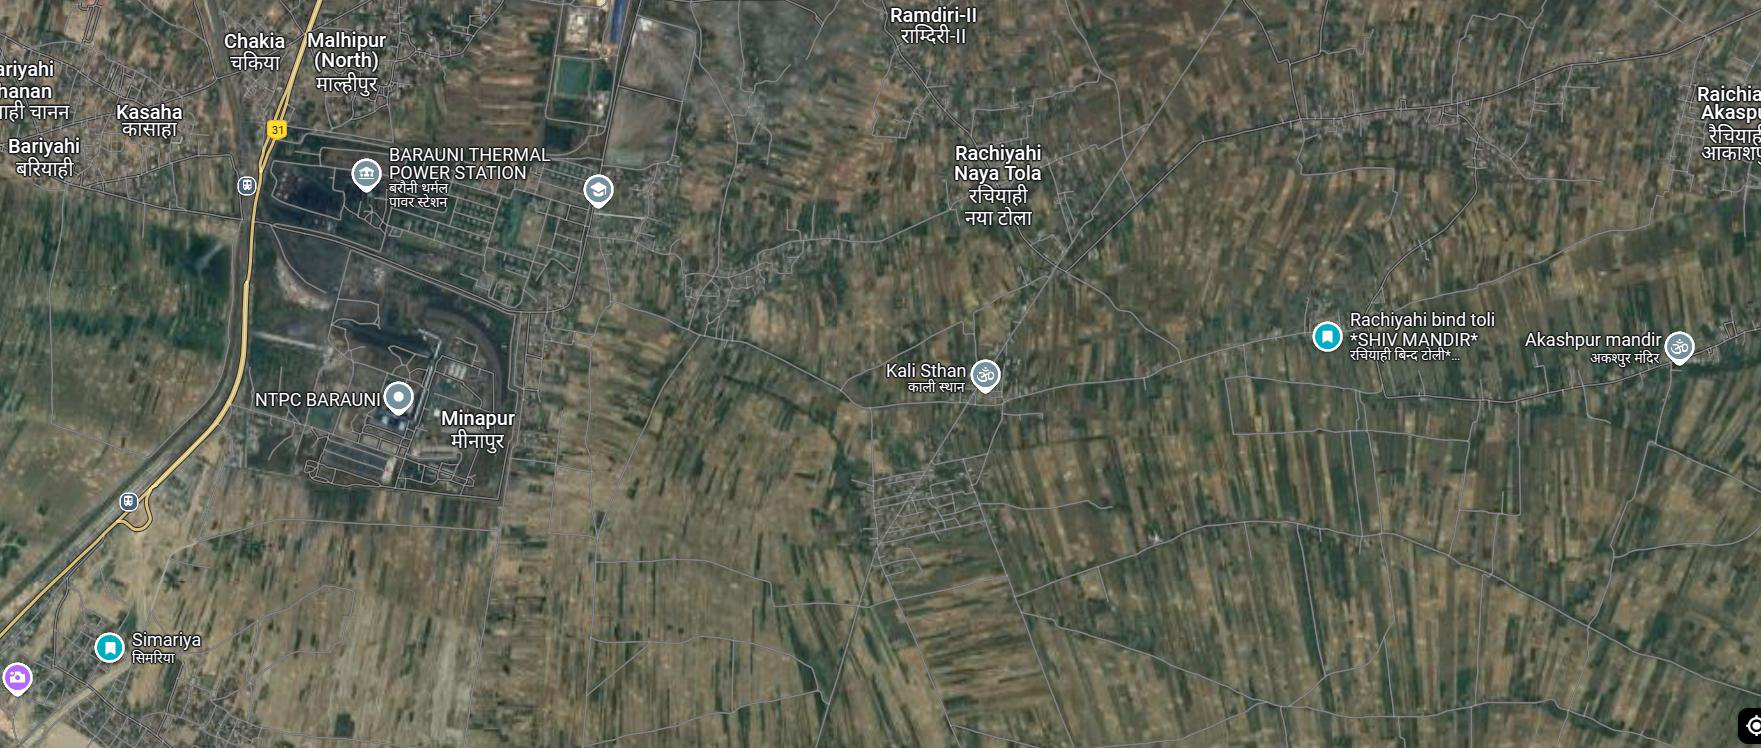
\includegraphics[width=0.8\textwidth]{fig_villages_along_route.png}
  \caption{Blue circle: IOCL Barauni industrial complex; red circles: villages affected by the
  alignment.}
\end{figure}

\section{Methodology (Design Process)}

\subsection{Design Criteria}
All candidate alignments considered, whether completed in full or explored preliminarily, are bypass
roads intended to divert traffic away from Begusarai's urban core.

\begin{itemize}
  \item \textbf{Design speed:} Alignment~1 is designed for 100~km/h, reflecting higher-speed industrial
  traffic flow; Alignments~2 and~3 are designed for 80~km/h, suitable for general bypass traffic.
  \item \textbf{Lane configuration:} Alignments~1 and~2 are 4-lane roads, sized for expected industrial
  vehicle volumes. Alignment~3 is a 2-lane road, since it passes through the Makor habitation area
  where land acquisition and environmental constraints necessitate a narrower cross-section.
  \item \textbf{Geometric design standards:} Both completed alignments follow IRC:73-1980 for horizontal
  and vertical curves, superelevation, and cross-section profile. Curve radii scale with design speed
  (larger radii for the 100~km/h alignment than for the 80~km/h alignment), and superelevation is
  computed from design speed and curve radius subject to a maximum rate of 7\%, per IRC:SP:84 for
  plain terrain.
  \item \textbf{Spiral length:} Spiral transitions of 70 to 90~m are used to provide smooth transitions
  between tangents and curves.
  \item \textbf{Traffic considerations:} Mixed traffic, comprising industrial vehicles, local traffic,
  and through traffic bypassing Begusarai, informs lane configuration and curve radii; heavier vehicles
  require wider curves and stronger superelevation for safety.
\end{itemize}

\subsection{Data Collection}
A Digital Elevation Model (DEM) provided the terrain data used for alignment creation in AutoCAD Civil
3D. The DEM was used to (i) generate terrain surfaces for accurate alignment modelling, (ii) analyse
elevation profiles and identify flood-prone areas near the Ganga river, and (iii) ensure the proposed
alignment respects natural landforms such as rivers, hillocks, and floodplains. In the absence of
direct traffic-count data for this coursework exercise, the DEM was the primary source of terrain and
elevation information guiding alignment placement.

\subsection{Civil 3D Model Development}
The alignment, profile, and cross-sections for Alignments~1 and~3 were developed in full in AutoCAD
Civil 3D following a standard corridor-design workflow; Alignment~2 was taken only as far as the
horizontal alignment and superelevation stages before design effort was concentrated on the two
alignments carried to completion:
\begin{center}
\small
DEM import $\rightarrow$ Horizontal alignment $\rightarrow$ Superelevation \& widening $\rightarrow$
Vertical alignment $\rightarrow$ Assembly $\rightarrow$ Corridor $\rightarrow$ Volume/earthwork calculation
\end{center}

\section{Alignment 1: Technical Details and Design Analysis}
Alignment~1 was designed to minimise travel time relative to the other alignments while keeping
cut-and-fill earthwork volumes low.

\begin{figure}[H]
  \centering
  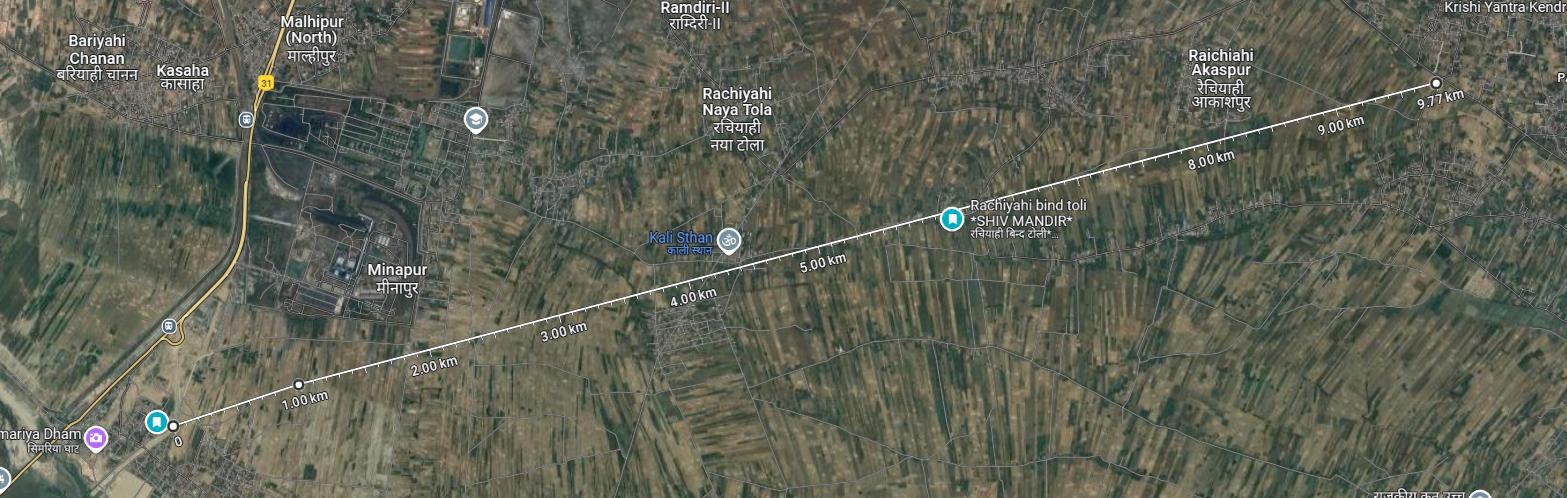
\includegraphics[width=0.85\textwidth]{fig_alignment1_route.png}
  \caption{Alignment 1: approximate origin-destination routing (Simaria, NH-31, to the undivided
  carriageway road near Matihani).}
\end{figure}

\begin{figure}[H]
  \centering
  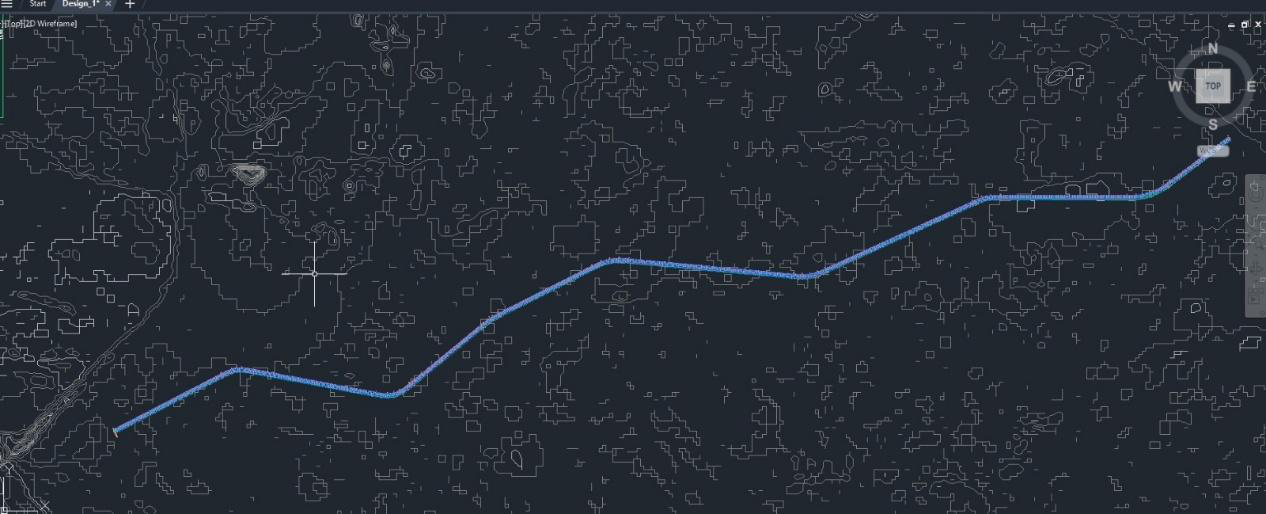
\includegraphics[width=0.7\textwidth]{fig_horizontal_alignment.png}
  \caption{Horizontal alignment of Alignment 1 in AutoCAD Civil 3D.}
\end{figure}

\begin{table}[H]
  \centering
  \caption{Technical parameters of Alignment 1.}
  \begin{tabular}{@{}ll@{}}
    \toprule
    \textbf{Parameter} & \textbf{Value} \\
    \midrule
    Design speed & 100 km/h \\
    Lane configuration & 4-lane divided \\
    Superelevation rate & 6\% \\
    Total curves & 7 \\
    Alignment length & 9.980 km \\
    Curve radius & 250 m \\
    Spiral length & 90 m \\
    Minimum spiral length & 45 m \\
    Spiral transition type & Spiral-in / Spiral-out \\
    Start station & 0+000.0 \\
    End station & 9+984.0 \\
    Elevation at start & 18.75 m \\
    Elevation at end & 17.50 m \\
    \bottomrule
  \end{tabular}
\end{table}

\subsection{Detailed Analysis of Design Variables}
Table~\ref{tab:geomdata} lists the full geometric-element table generated by Civil~3D for Alignment~1:
each tangent (line) and spiral-curve-spiral group, its length, spiral parameters, radius, and degree of
curvature. Line elements are unconstrained (fixed, defined by two points); spiral-curve-spiral elements
are constrained on both sides (free), parameterised as spiral-in, radius, spiral-out. The design-speed
field in the Civil~3D template records 80~km/h throughout this table, reflecting the software's default
alignment-creation parameter rather than the 100~km/h target design speed discussed for Alignment~1
elsewhere in this report.

\begin{longtable}{p{0.9cm}p{1.6cm}p{1.5cm}p{1.7cm}p{1.4cm}p{1.5cm}p{1.4cm}p{1.6cm}}
\caption{Geometric design data for Alignment 1 (tangent/spiral/curve elements, as generated in Civil 3D).}
\label{tab:geomdata} \\
\toprule
\textbf{No.} & \textbf{Element} & \textbf{Length (m)} & \textbf{Min.\ spiral (m)} & \textbf{Radius (m)} & \textbf{Min.\ radius (m)} & \textbf{A} & \textbf{Degree of curv.} \\
\midrule
\endfirsthead
\toprule
\textbf{No.} & \textbf{Element} & \textbf{Length (m)} & \textbf{Min.\ spiral (m)} & \textbf{Radius (m)} & \textbf{Min.\ radius (m)} & \textbf{A} & \textbf{Degree of curv.} \\
\midrule
\endhead
\bottomrule
\endfoot
1 & Line & 1003.743 & -- & -- & -- & -- & -- \\
2.1 & Spiral-in & 90.000 & 90.000 & -- & -- & 150.000 & -- \\
2.2 & Curve & 75.699 & -- & 250.000 & 250.000 & -- & 6.9855 \\
2.3 & Spiral-out & 90.000 & 90.000 & -- & -- & 150.000 & -- \\
3 & Line & 1037.481 & -- & -- & -- & -- & -- \\
4.1 & Spiral-in & 100.000 & 90.000 & -- & -- & 158.114 & -- \\
4.2 & Curve & 118.393 & -- & 250.000 & 250.000 & -- & 6.9855 \\
4.3 & Spiral-out & 100.000 & 90.000 & -- & -- & 158.114 & -- \\
5 & Line & 769.374 & -- & -- & -- & -- & -- \\
6.1 & Spiral-in & 60.000 & 45.000 & -- & -- & 173.205 & -- \\
6.2 & Curve & 49.689 & -- & 500.000 & 250.000 & -- & 3.4928 \\
6.3 & Spiral-out & 60.000 & 45.000 & -- & -- & 173.205 & -- \\
7 & Line & 862.321 & -- & -- & -- & -- & -- \\
8.1 & Spiral-in & 80.000 & 55.000 & -- & -- & 178.885 & -- \\
8.2 & Curve & 144.674 & -- & 400.000 & 250.000 & -- & 4.3659 \\
8.3 & Spiral-out & 80.000 & 55.000 & -- & -- & 178.885 & -- \\
9 & Line & 1368.077 & -- & -- & -- & -- & -- \\
10.1 & Spiral-in & 70.000 & 55.000 & -- & -- & 167.332 & -- \\
10.2 & Curve & 138.469 & -- & 400.000 & 250.000 & -- & 4.3659 \\
10.3 & Spiral-out & 70.000 & 55.000 & -- & -- & 167.332 & -- \\
11 & Line & 1338.740 & -- & -- & -- & -- & -- \\
12.1 & Spiral-in & 80.000 & 60.000 & -- & -- & 167.332 & -- \\
12.2 & Curve & 69.991 & -- & 350.000 & 250.000 & -- & 4.9896 \\
12.3 & Spiral-out & 80.000 & 60.000 & -- & -- & 167.332 & -- \\
13 & Line & 1042.366 & -- & -- & -- & -- & -- \\
14.1 & Spiral-in & 80.000 & 45.000 & -- & -- & 200.000 & -- \\
14.2 & Curve & 242.831 & -- & 500.000 & 250.000 & -- & 3.4928 \\
14.3 & Spiral-out & 80.000 & 45.000 & -- & -- & 200.000 & -- \\
15 & Line & 602.215 & -- & -- & -- & -- & -- \\
\end{longtable}

\textbf{Superelevation.} For the 100~km/h design speed, superelevation is calculated at a 6\% rate and
applied symmetrically on both lanes of the 4-lane divided cross-section.

\begin{figure}[H]
  \centering
  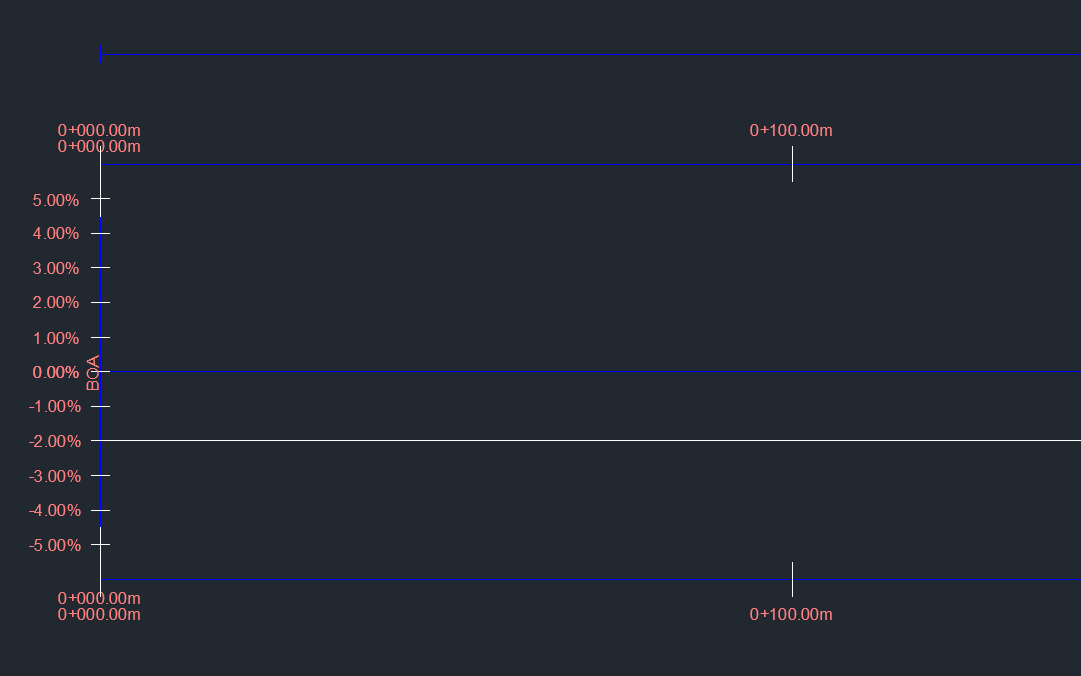
\includegraphics[width=0.55\textwidth]{fig_superelevation_curve1.png}
  \caption{Superelevation transition for Curve 1 of Alignment 1.}
\end{figure}

\begin{figure}[H]
  \centering
  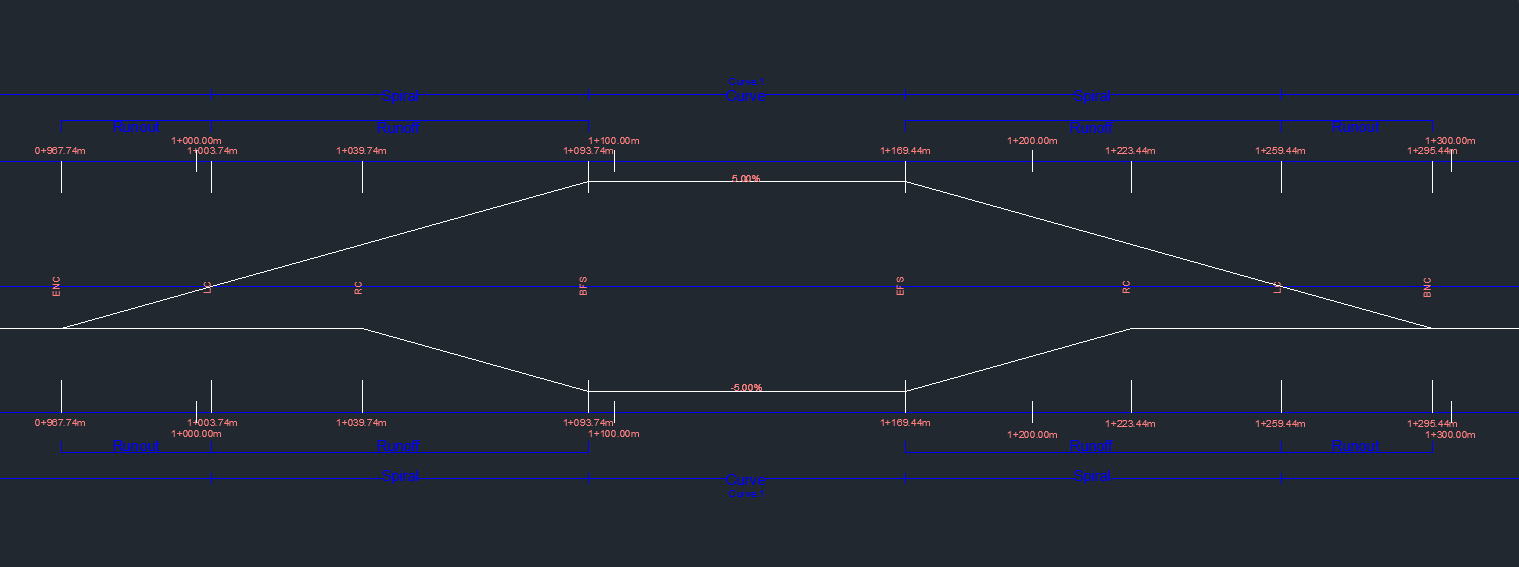
\includegraphics[width=0.85\textwidth]{fig_superelevation_diagram.png}
  \caption{Full superelevation diagram along Alignment 1, showing runoff and runout zones either side
  of each curve.}
\end{figure}

\textbf{Curve radius.} The 250~m curve radius adopted for Alignment~1 provides a smooth turning path
suitable for the 100~km/h design speed and is within acceptable limits for high-speed highway design.

\begin{figure}[H]
  \centering
  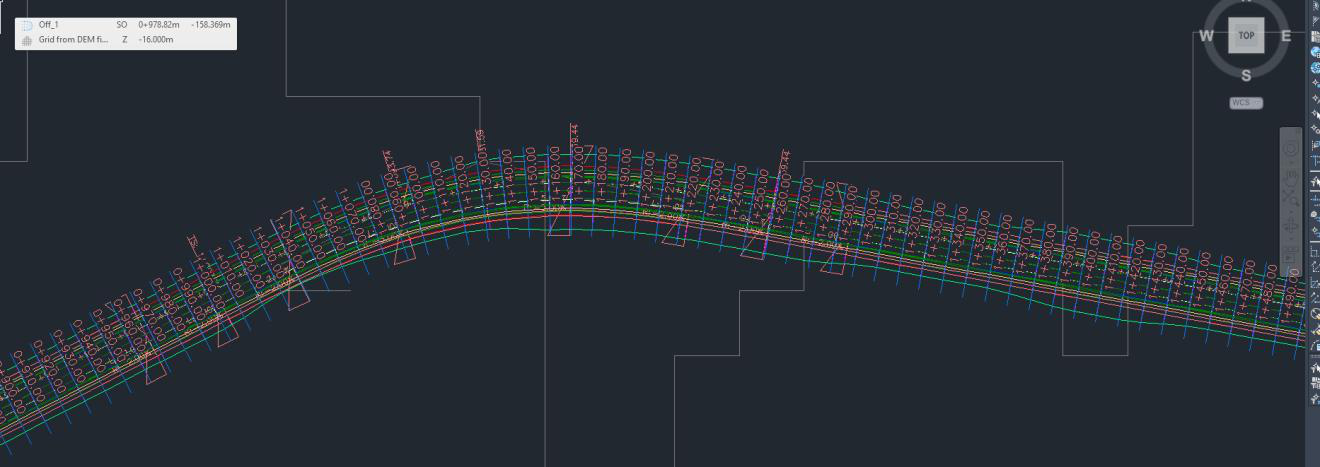
\includegraphics[width=0.85\textwidth]{fig_corridor_generation.png}
  \caption{Corridor model generated along a representative curve of Alignment 1.}
\end{figure}

\textbf{Spiral length.} A 90~m spiral length provides a smooth tangent-to-curve transition, reducing
the rate of change of lateral acceleration (jerk) felt by drivers, particularly in high-speed zones;
sharper transitions use extended spiral lengths to avoid abrupt superelevation changes.

\subsection{Geometric Design Evaluation}
\textbf{Horizontal alignment.} The horizontal alignment follows the natural terrain to minimise land
acquisition, with curves spaced to allow heavy industrial and mixed traffic to flow without conflict.

\textbf{Vertical alignment.} Vertical grades meet IRC guidelines, keeping the maximum gradient within
4\% for high-speed roads and avoiding sharp elevation changes in favour of a smooth longitudinal
profile.

\begin{figure}[H]
  \centering
  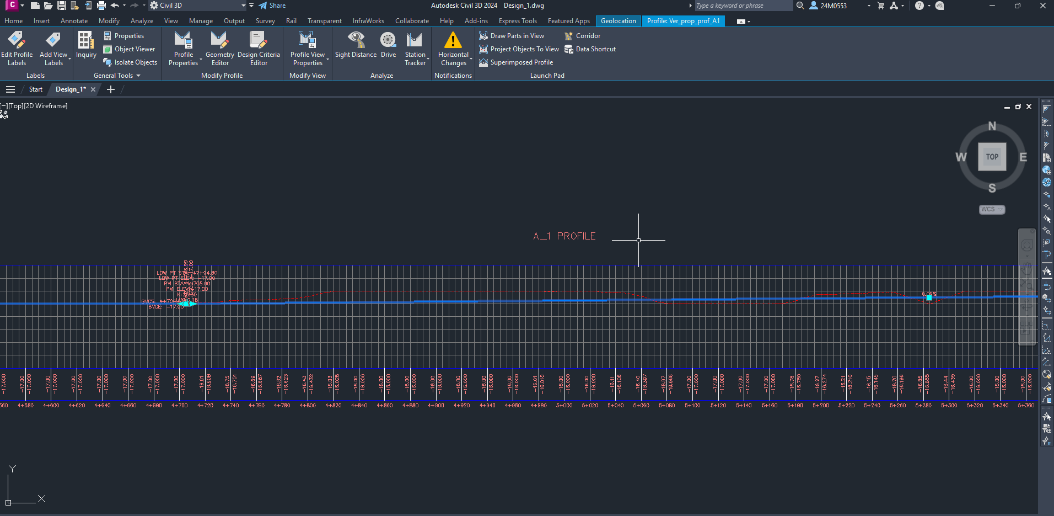
\includegraphics[width=0.55\textwidth]{fig_vertical_alignment.png}
  \caption{Vertical alignment profile for Alignment 1 in Civil 3D.}
\end{figure}

\textbf{Cross-section design.} The 4-lane cross-section provides 3.5~m lane widths (the Indian highway
standard) and a 2.5~m shoulder for emergency stops and service vehicles, giving adequate width for
mixed light-vehicle and heavy-truck traffic without congestion.

\subsection{Cut-and-Fill Analysis}
Earthwork quantities were computed from the DEM-derived terrain surface. The alignment required
elevated (embanked) sections near Bind Toli to account for flood-prone areas close to the Ganga river.
Table~\ref{tab:volume1} shows a representative excerpt of the station-by-station volume report
generated in Civil 3D; the cumulative net earthwork volume at the final station (9+980.000) was
approximately 129{,}634~m\textsuperscript{3}.

\begin{table}[H]
  \centering
  \small
  \caption{Excerpt of the cut/fill volume report for Alignment 1 (Start Sta.\ 0+010, End Sta.\ 9+980). All areas in m\textsuperscript{2}, all volumes in m\textsuperscript{3}.}
  \label{tab:volume1}
  \begin{tabular}{@{}rrrrrr@{}}
    \toprule
    \textbf{Station} & \textbf{Cut area} & \textbf{Cut vol.} & \textbf{Fill area} & \textbf{Fill vol.} & \textbf{Cum.\ net vol.} \\
    \midrule
    0+010.000 & 10.78 & 0.00   & 0.00  & 0.00   & 0.00 \\
    0+050.000 & 10.78 & 107.76 & 0.00  & 0.00   & 538.82 \\
    0+100.000 & 10.78 & 107.76 & 0.00  & 0.00   & 969.87 \\
    0+180.000 & 3.30  & 49.60  & 6.67  & 44.77  & 1689.55 \\
    9+800.000 & 27.89 & 256.90 & 0.00  & 0.00   & 126027.90 \\
    9+900.000 & 20.40 & 203.08 & 0.00  & 0.00   & 128773.17 \\
    9+980.000 & 9.06  & 85.30  & 0.54  & 7.08   & 129633.83 \\
    \bottomrule
  \end{tabular}
\end{table}

\section{Alignment 2: Preliminary Exploration (Not Carried Forward)}
Alignment~2 is similar to Alignment~1 in origin, destination, and 4-lane cross-section, differing
primarily in total length as a result of a slightly different routing through the terrain. This option
was explored preliminarily in Civil 3D, with horizontal routing and a superelevation diagram generated
as shown below, but given the time available for this coursework project, detailed corridor modelling
and earthwork quantification were not carried out for this alignment. Design effort was instead
concentrated on Alignments~1 and~3, which are presented in full in this report.

\begin{figure}[H]
  \centering
  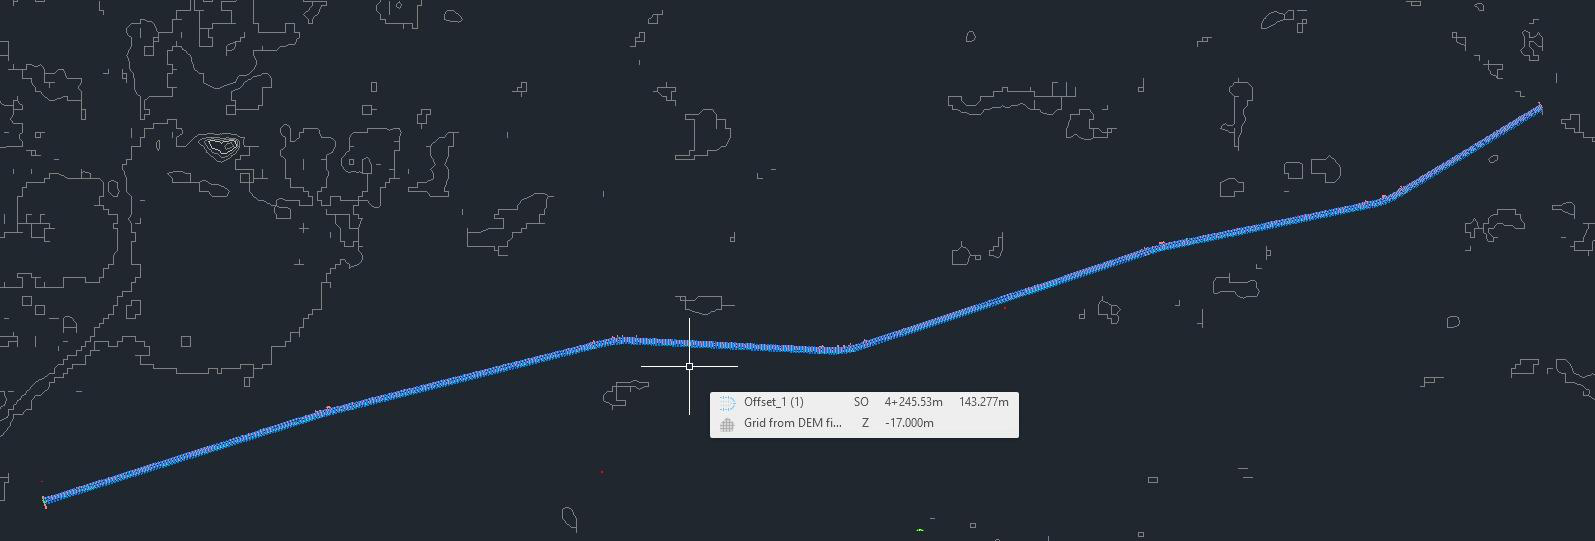
\includegraphics[width=0.8\textwidth]{fig_alignment2_route.png}
  \caption{Alignment 2 routing over the DEM-derived terrain grid.}
\end{figure}

\begin{figure}[H]
  \centering
  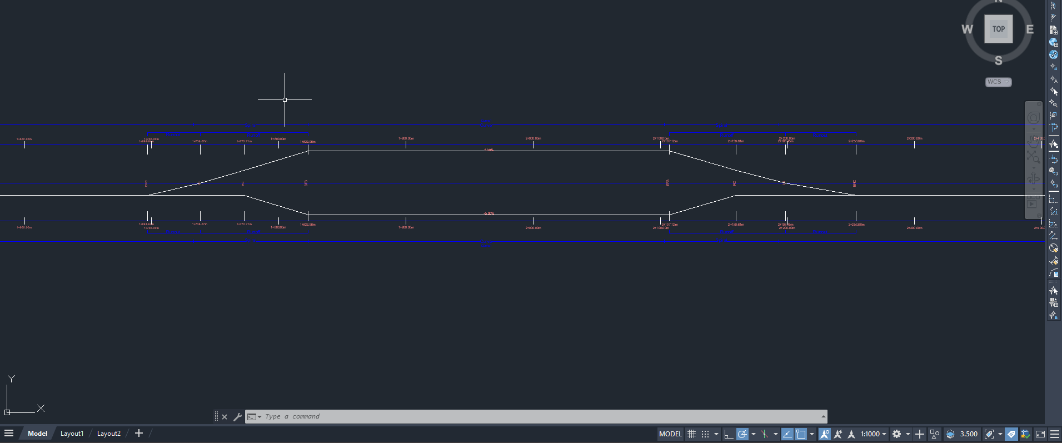
\includegraphics[width=0.75\textwidth]{fig_alignment2_superelevation.png}
  \caption{Superelevation diagram for Alignment 2.}
\end{figure}

\section{Alignment 3: 2-Lane Village Connector}
Alignment~3 was designed as a 2-lane, 80~km/h bypass connecting Bind Toli and other scattered villages
before merging with the existing undivided carriageway. Because it passes through the Makor
habitation area, its narrower 2-lane cross-section reflects land-acquisition and environmental
constraints rather than a lower expected traffic volume.

\begin{figure}[H]
  \centering
  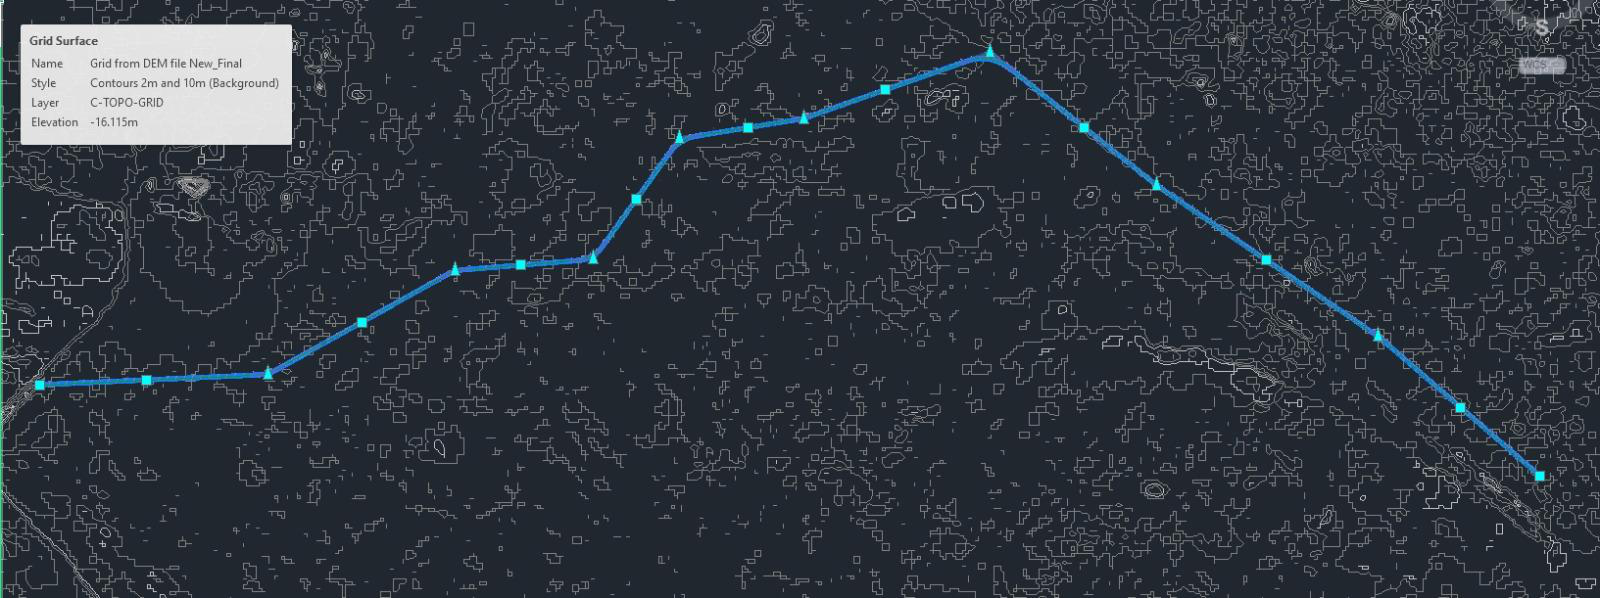
\includegraphics[width=0.85\textwidth]{fig_alignment3_route.png}
  \caption{Alignment 3 routing, connecting village areas before widening at the final curve.}
\end{figure}

\begin{table}[H]
  \centering
  \caption{Design variables for Alignment 3.}
  \begin{tabular}{@{}ll@{}}
    \toprule
    \textbf{Parameter} & \textbf{Value} \\
    \midrule
    Design speed & 80 km/h \\
    Alignment length & 15.66 km \\
    Lane configuration & 2-lane road \\
    Superelevation rate & 4--5\% (depending on the curve) \\
    Curve radius & 200 m to 500 m \\
    Total curves & 9 \\
    Spiral length & 45 m -- 90 m \\
    Minimum spiral length & 45 m \\
    Start station & 0+000.0 \\
    End station & 15+000.0 \\
    Spiral type & Spiral-in / Spiral-out \\
    Earthwork & Cut and fill based on DEM data \\
    \bottomrule
  \end{tabular}
\end{table}

\begin{figure}[H]
  \centering
  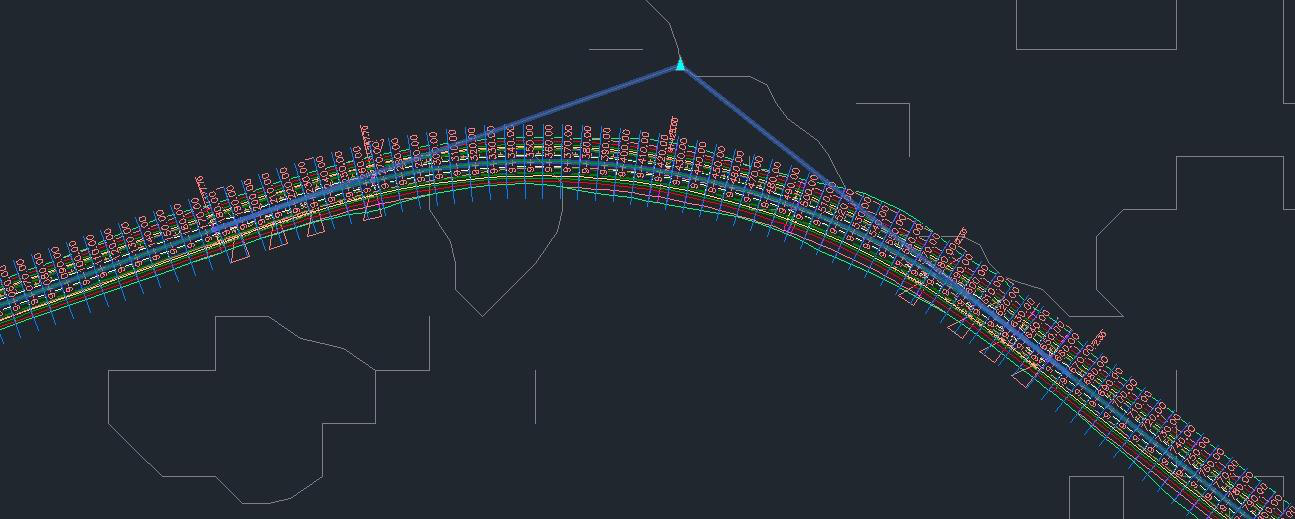
\includegraphics[width=0.85\textwidth]{fig_alignment3_corridor.png}
  \caption{Corridor model along a representative curve of Alignment 3.}
\end{figure}

The cut-and-fill volume report for Alignment~3 (Start Sta.\ 0+010, End Sta.\ 15+660) shows a
cumulative net earthwork volume of approximately 293{,}198~m\textsuperscript{3} at the final station,
reflecting the longer alignment length and the more undulating terrain traversed relative to
Alignment~1.

\section{Discussion}
The two completed alignments illustrate a set of trade-offs typical of greenfield bypass design.
Alignment~1, designed for 100~km/h with 250~m curve radii, minimises travel time for industrial and
through traffic at the cost of a wider 4-lane cross-section and larger land take. Alignment~3 trades
capacity (2 lanes instead of 4) and a lower nominal design speed for a routing that minimises impact on
the Makor habitation area, at the expense of a longer overall length (15.66~km versus 9.98~km for
Alignment~1) and correspondingly larger cumulative earthwork volumes. A third option, Alignment~2,
offering similar 4-lane capacity to Alignment~1 at a more conservative 80~km/h design speed, was
explored at the routing and superelevation stage but was not carried through to full corridor design
and earthwork quantification within the time available for this project. For both completed
alignments, adherence to IRC:73-1980 curve-radius and superelevation limits, together with
DEM-informed vertical design, ensures the alignments remain constructible on the flood-prone,
low-relief terrain characteristic of the Simaria--Matihani corridor near the Ganga river.

\section{Conclusion}
This project successfully achieved:
\begin{itemize}
  \item Terrain modelling using real DEM/satellite data;
  \item Engineering-grade horizontal alignment creation for two fully designed candidate bypass routes
  (Alignments~1 and~3), with a third option (Alignment~2) explored preliminarily;
  \item Compliance with Indian geometric design standards (IRC:73-1980, IRC:SP:84);
  \item A policy-aligned justification for bypass development, linking the design directly to the
  stated regional objectives of decongesting NH-31 and improving industrial and agricultural
  connectivity around Begusarai.
\end{itemize}
This design work lays the groundwork for the subsequent stages of a fully implementable bypass design,
namely refined vertical profiling, detailed superelevation and widening design, corridor modelling, and
earthwork-based cost estimation, all of which were carried out for Alignments~1 and~3 in this report.

\begin{thebibliography}{9}
\bibitem{irc73} Indian Roads Congress. \textit{IRC:73-1980 -- Geometric Design Standards for Rural
(Non-Urban) Highways}.
\bibitem{ircsp84} Indian Roads Congress. \textit{IRC:SP:84 -- Manual of Specifications and Standards
for Six Laning of Highways}.
\end{thebibliography}

\end{document}
